\section{OTP - Open Telecom Platform}

L'OTP (Open Telecom Platform) è stato sviluppato
da Ericsson negli anni '80 come insieme di strumenti,
librerie e standard per affrontare le sfide specifiche
del settore delle telecomunicazioni,
come l'affidabilità e la tolleranza agli errori.

Basato sul linguaggio di programmazione Erlang,
OTP è stato progettato per gestire la concorrenza
e le comunicazioni asincrone,
rendendolo ideale per sistemi distribuiti.
Nel corso degli anni, l'OTP ha trovato applicazioni
anche in altri settori, diventando una scelta popolare
per sistemi altamente affidabili e scalabili.

Elixir fornisce un'interfaccia più moderna e una sintassi
più chiara rispetto ad Erlang, mantenendo al tempo stesso
la potenza e l'affidabilità di Erlang e OTP.

Per quanto riguarda il mentanimento di uno
stato, in Elixir si può fare affidamento ai Behaviour
Agent e GenServer, consentendo di dare la responsabilità
al mantenimento di uno stato ad un altro processo.

ci consentono di mantenere uno stato senza dover reinventare la
ruota nello scrivere un modulo soltanto per farlo.
L'approccio nella programmazione è totalmente differente
e piuttosto singolare rispetto ai più comuni linguaggi di programmazione,
ma è proprio questa singolarità che può porta il linguaggio
ad essere orientato alla concorrenza. 

%---------------------------------------------------------------------------------

\subsection{GenServer}
Per mantenere uno stato si potrebbe scrivere un modulo che
tramite le primitive concorrenziali gestiscono lo stato
a piacimento. Elixir però mette a disposizione il Behaviour
GenServer, un OTP server è un modulo con il
"Behaviour" GenServer.
Il "Behaviour" è un meccanismo che consente di definire
uno schema comune per un tipo specifico di processo.

Ad esempio il GenServer Behaviour definisce le funzioni e
le interfacce necessarie per creare un processo server in grado
di gestire le richieste in modo asincrono.
Utilizzando il GenServer Behaviour, è possibile definire i comportamenti
di base del server e personalizzarli secondo le esigenze specifiche
dell'applicazione. 
Questo fornisce un alto livello di astrazione per la gestione
dei processi e semplifica lo sviluppo di sistemi concorrenti e
distribuiti in Elixir.

Il vantaggio di utilizzare un GenServer è che ha un'insieme
di interfacce standard e include funzionalità di tracciamento
e segnalazione degli errori. Si può anche mettere dentro un
albero di supervisione.

Questo Behaviour astrae l'interazione Client-server, come si può vedere
in figura \ref{fig:client_server}  \cite{GenServe6:online},
lo stato è gestito dal Server, e i processi client sono quelli che
devono modificare lo stato o accedere ad esso.

\begin{figure}[!htp]
    \centering
    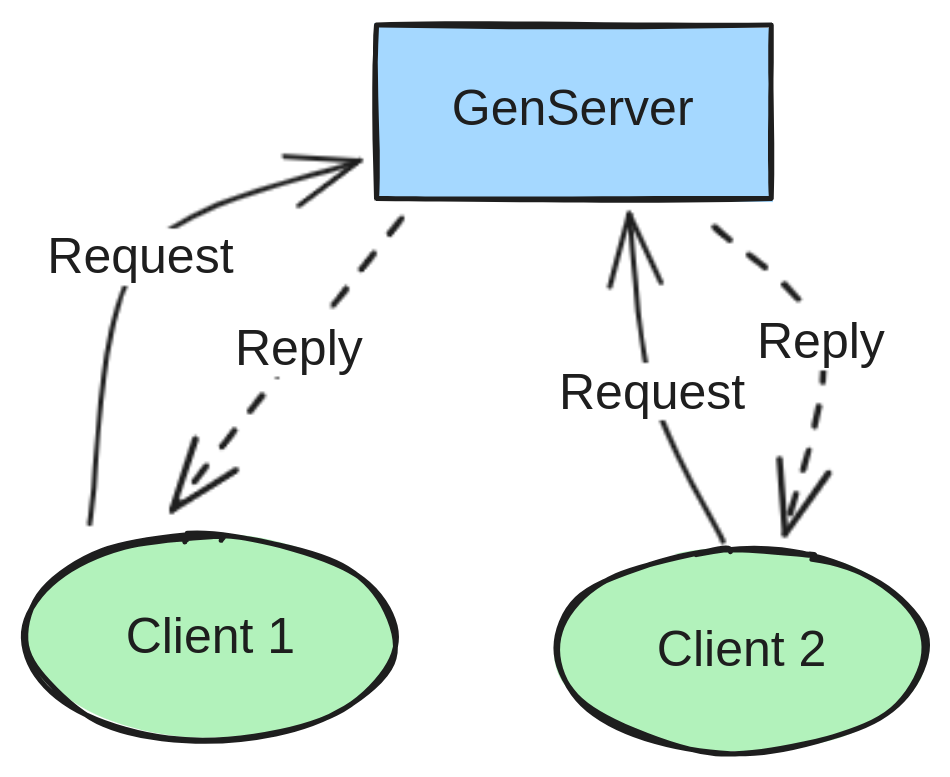
\includegraphics[keepaspectratio=true,scale=0.20]{images/GenServer.png}
	\caption{Interazione Client-Server}
  	\label{fig:client_server}
\end{figure}

Per implementare il behaviour GenServer, bisogna affidarsi alla
documentazione di GenServer, in particolare vanno ridefinite delle
callback, ed ogni funzione può restituire un determinato insieme di
strutture dati.

Nell'esempio \ref{lst:stackGenServer} viene implementata una struttura dati
per mantere uno Stack di dati \cite{GenServe6:online}.

\begin{lstlisting}[language=elixir, caption={Implementazione Stack},captionpos=b,
	label={lst:stackGenServer}]
defmodule Stack do
use GenServer

# Client

def start_link(default) when is_binary(default) do
  GenServer.start_link(__MODULE__, default)
end

def push(pid, element) do
  GenServer.cast(pid, {:push, element})
end

def pop(pid) do
  GenServer.call(pid, :pop)
end

# Server (callbacks)

@impl true
def init(elements) do
  initial_state = String.split(elements, ",", trim: true)
  {:ok, initial_state}
end

@impl true
def handle_call(:pop, _from, state) do
  [to_caller | new_state] = state
  {:reply, to_caller, new_state}
end

@impl true
def handle_cast({:push, element}, state) do
  new_state = [element | state]
  {:noreply, new_state}
end
  end
\end{lstlisting}

Nell'esempio possiamo vedere che il modulo stack implementa
la funzione \textbf{init/1} che inizializza lo stato con gli elementi
iniziali quando il server viene avviato, la funzione \textbf{handle\_call/3}
chiamata per le operazioni di :pop dello stack,
è una funzione sincrona, quindi viene usata quando ci si aspetta
un valore di ritorno, infatti restituisce il valore di
testa dello stack. La funzione \textbf{handle\_cast/2} invece viene usata per
le operazioni asincrone, quindi nel caso in esame per l'operazione di
push nello Stack che non necessita di risposta.

Quindi il GenServer è un'astrazione che:

\begin{itemize}
	\item Incapsula un servizio condiviso.
	\item Mantiene uno stato.
	\item Permette un'astrazione concorrente ad un servizio condiviso \cite{adoptingElixirchap5pag96}.
\end{itemize}

%---------------------------------------------------------------------------------

\subsection{Supervisor}

Un'altro concetto cardine dell'OTP è il Supervisor con cui si
riesce a raggiungere un alto livello di Fault-tolerant.

Il compito principale di un supervisor è quello di monitorare,
controllare e gestire il ciclo di vita dei processi all'interno
di un sistema Erlang o Elixir. I supervisori sono 
particolarmente utili per garantire la stabilità e 
l'affidabilità dei sistemi distribuiti, poiché gestiscono 
automaticamente il riavvio dei processi in caso di fallimenti, 
garantendo che il sistema continui a funzionare anche in
situazioni critiche.

In pratica come il GenServer, un  Supervisor è un modulo
che implementa il Behaviour Supervisor.

\newpage

Ci sono diversi tipi di Supervisor in Erlang ed Elixir, tra cui:
\begin{itemize}
  \item \textbf{Supervisor Semplice}: Questi supervisori monitorano
  direttamente i processi figlio e li riavviano se necessario.
  Sono utilizzati per gestire processi che non hanno stati interni
  o che devono essere riavviati senza alcuna elaborazione specifica.
  \item \textbf{Supervisori gerarchici}: Questi supervisori controllano
  una gerarchia di altri supervisori e processi.
  Possono essere configurati per riavviare solo parti
  specifiche del sistema in caso di problemi,
  consentendo un maggiore controllo sul comportamento di riavvio.
  \item \textbf{Supervisori dinamici}: Questi supervisori possono
  essere creati e configurati dinamicamente durante l'esecuzione
  del programma, consentendo una maggiore flessibilità
  nell'aggiunta e nella gestione dei processi.


 
\end{itemize}

Per implementare un Supervisor di deve decidere quali sono i processi
figli da supervisionare, e si avvia il Supervisor
con la funzione \textbf{start\_link/2}
Bisogna quindi decidere quali sono i processi figli da supervisionare,
e una volta avviato il Supervisor con la funzione \textbf{start\_link/2},
questo ha bisogno di sapere come avviare, fermare o riavviare i suoi figli
in caso di errore o uscita imprevista.

Una volta avviato il Supervisor, deve sapere come fare lo start/stop/restart
dei suoi figli da monitorare. Per questo i moduli da supervisionare
devono implementare una funzione che definisce le specifiche,
la funzione in questione è \textbf{child\_spec/1},
restituisce una Map per
configurare il comportamento in caso di supervisione.

Alcuni moduli come il GenServer già definiscono questa funzione
non avendo la necessità di ridefinirla, come il GenServer e
il modulo Task che utilizzeremo successivamente.
